\aufgabenbereich{Computer Architektur}
\subsection{}
\subsubsection{}
Was ist der Unterschied zwischen einer Harvard und einer Van-Neumann-Architektur?\\
\makeanswerbox{5}
\subsubsection{}
Listen sie die Operationen die ein ALU durchführen kann:
\def\dist{11cm}
\begin{itemize}
	\item \makeinlineanswerbox{5}{\dist}
	\item \makeinlineanswerbox{5}{\dist}
	\item \makeinlineanswerbox{5}{\dist}
	\item \makeinlineanswerbox{5}{\dist}
	\item \makeinlineanswerbox{5}{\dist}
	\item \makeinlineanswerbox{5}{\dist}
\end{itemize}
\newpage\noindent
\subsubsection{}
Welche Operation kann die Function Unit neben den Funktionen der ALU auch durchführen?
\begin{itemize}
	\item \makeinlineanswerbox{5}{\dist}
	\item \makeinlineanswerbox{5}{\dist}
	\item \makeinlineanswerbox{5}{\dist}
	\item \makeinlineanswerbox{5}{\dist}
\end{itemize} 
(Hinweis: Sie müssen nicht alle Felder ausfüllen für die korrekte Antwort.)
\subsection{Kontrollpfad}
Nennen Sie die einzelnen Schritte einer Befehlsausführung:
\begin{enumerate}
	\item \makeinlineanswerbox{5}{\dist}
	\item \makeinlineanswerbox{5}{\dist}
	\item \makeinlineanswerbox{5}{\dist}
	\item \makeinlineanswerbox{5}{\dist}
	\item \makeinlineanswerbox{5}{\dist}
	\item \makeinlineanswerbox{5}{\dist}
\end{enumerate}
\subsection{Datenpfad}
Erklären Sie kurz wie der Datenpfad in einem Prozessor aussieht:\\
\makeanswerbox{8}
\subsection{Befehlsformat}
Geben Sie ein Befehlsformat für Assembler Befehle an. Beschriften sie die Blöcke mit ihrer Bitgröße:
\begin{center}
	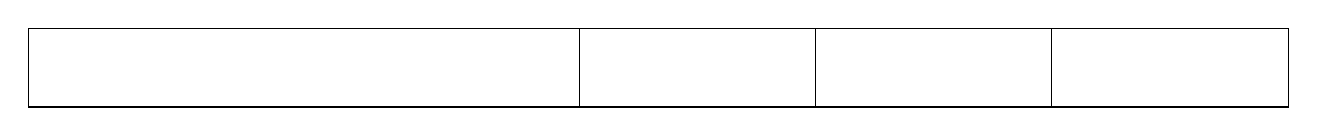
\begin{tikzpicture}
	\draw (0,0) rectangle (16,1);
	\draw (0,0) rectangle (7,1);
	\draw (7,0) rectangle (10,1);
	\draw (10,0) rectangle (13,1);
	\draw (13,0) rectangle (16,1);
	\end{tikzpicture}
\end{center}
\subsection{Flags}
Beschreiben Sie die Funktion von folgenden Flags:\\
$
\begin{array}{r l}
	C: & \begin{minipage}{0.9\textwidth}
		\makeanswerbox{1.5}
	\end{minipage}\\
	O: & \begin{minipage}{0.93\textwidth}
	\makeanswerbox{1.5}
	\end{minipage}\\
	N: & \begin{minipage}{0.93\textwidth}
	\makeanswerbox{1.5}
	\end{minipage}\\
	Z: & \begin{minipage}{0.93\textwidth}
	\makeanswerbox{1.5}
	\end{minipage}\\
\end{array}.
$\\
Wo werden diese Flags erzeugt?\\
\makeanswerbox{2}
